
\documentclass[a4paper,10pt, spanish]{article}
\usepackage{caratula}
\usepackage[spanish]{babel}
\usepackage{amsmath}
%\usepackage{algorithm}
\usepackage[spanish,onelanguage]{algorithm2e}
\usepackage[noend]{algpseudocode}
%\selectlanguage{spanish}
%% The graphicx package provides the includegraphics command.
\usepackage{graphicx}
%% The amssymb package provides various useful mathematical symbols
\usepackage{amssymb}
\usepackage{caption}

\usepackage[T1]{fontenc}
\usepackage{selinput}
\SelectInputMappings{%
  aacute={á},
  ntilde={ñ},
}

% Espaciado entre parrafos
\setlength{\parskip}{1mm}
  
%% The lineno packages adds line numbers. Start line numbering with
%% \begin{linenumbers}, end it with \end{linenumbers}. Or switch it on
%% for the whole article with \linenumbers after \end{frontmatter}.
\usepackage{lineno}

\author{}
\date{}
\title{Trabajo pr\'actico III}

\def\Materia{Algoritmos y Estructuras de Datos III}
\def\Titulo{Trabajo pr\'actico III}


\integrante{Delger, Agust\'in}{274/14}{agusdel\_94@hotmail.com}
\integrante{Delmagro, Nicolás Agust\'in}{596/14}{agustin.delmagro@gmail.com}
\integrante{Lopez Valiente, Patricio}{457/15}{patricio454@gmail.com}
\integrante{Zar Abad, Ciro Román}{129/15}{ciromanzar@gmail.com}

\begin{document}
\maketitle

\tableofcontents
\newpage

\section{Introducción}
En este trabajo se analiza el problema de \textit{clique de máxima frontera} (CMF). Para definir en qué consiste este problema, primero es necesario definir el término \textit{clique} y luego su \textit{frontera}.

Dado un grafo simple $G$ = ($V, E$), un subconjunto de vértices de $G$ es una \textit{clique} si y sólo si éste induce
un subgrafo completo de $G$. Es decir, $K \subseteq V$, tal que $K \neq \emptyset$, es una clique de $G$ si y sólo si para todo
par de vértices $u, v \in K, u \neq v$, existe la arista $(u,v)$ en $E$.

Definimos la \textit{frontera} de una clique $K$ como el
conjunto de aristas de $G$ que tienen un extremo en $K$ y otro en $V \setminus K$. Formalmente, la frontera de una
clique $K$ queda definida por

$\delta(K) = \lbrace (v,w) \in E / v \in K \wedge w \in V \setminus K \rbrace$.

Una vez definido esto, el problema de clique de máxima frontera (CMF) en un grafo $G$ consiste en hallar una clique $K$ de $G$ cuya frontera $\delta$(K) tenga cardinalidad máxima. Algunas situaciones de la vida real que pueden ser modelados a través de este problema se pueden ver en la sección siguiente.

Si bien CMF es un problema conocido, no se conocen algoritmos polinomiales que lo resuelvan. En este trabajo, primero se resolverá el problema de forma exacta, utilizando la técnica \textit{Backtracking}. Luego, con el fin de mejorar la complejidad, se presentarán varios algoritmos heurísticos que también intenten resolverlo.

En concreto, se implementarán los siguientes algoritmos:

\begin{enumerate}
\item Un algoritmo exacto utilizando \textit{Backtracking}.
\item Dos heurísticas constructivas \textit{golosas}.
\item Una heurística de \textit{búsqueda local}.
\item Una heurística \textit{GRASP}.
\end{enumerate}

El objetivo de este trabajo es experimentar sobre cada uno de los algoritmos implementados, estudiando su complejidad y tiempo de ejecución en función del tamaño de la entrada, y, en los algoritmos heurísticos, también analizar la calidad de los datos. Se intentarán definir familias de grafos que optimicen los resultados, o que hagan los contrario, es decir, que no proporcionen una solución óptima. 
\newpage

\section{Situación real modelada con CMF}
\subsection{Pinche Trump Cat Problem}
Los Estados Unidos de América acaban de invadir México y el emperador Ronald Trump decidió que su nuevo territorio necesita con urgencia una reestructuración politica completa. 

Una de las primeras medidas a tomar es cambiar la distribución de las provincias del pais, y en particular mudar la capital administrativa de México D.F. a un territorio denominado Centro de Reinado de México (CRM). Este territorio puede estar formado por una o más ciudades y debe cumplir con los siquientes requerimientos estrictos:

\begin{itemize}
\item Todas las ciudades dentro del territorio deben estar conectadas entre sí por rutas directas (es decir sin pasar por otras ciudades intermedias), para asegurar una fluida comunicación.
\item Dichas ciudades tienen que tener la mayor cantidad posible de rutas que comuniquen el CRM con ciudades fuera de este, para favorecer el comercio interno pero principalmente para proveer vias de escape en caso de atentados terroristas realizados contra su Deidad Gobernante.
\item No es problema si dentro del territorio delimitado queda alguna ciudad que no cumpla el primer punto, ya que estas pueden formar parte de otras provincias dentro del CRM.
\end{itemize}

Roland Trump decidió contratar (en un intento por corregir la imagen pública de xenófobo que le fue injustamente atribuida) a un equipo de latinos del Departamento de Computación de la UBA, en Argentina, para determinar la mejor ubicación del CRM.

Para resolver este problema, el territorio mexicano puede ser representado como un grafo, donde los nodos son las ciudades y existe una arista entre ellos si hay alguna ruta directa que conecte estas ciudades.

Por lo tanto, la nueva capital administrativa será una clique en nuestro grafo ya que es condición necesaria que todas las ciudades dentro del CRM se conecten entre sí, es decir, que exista una arista entre ellas. Además, de todas las cliques posibles del grafo debe de ser una de las cliques (ya que puede existir más de una) que tenga mayor cantidad de aristas que conecten a los nodos de la clique con los que no pertenecen a ésta. Esto se debe a que se busca maximizar las rutas que conectan a la nueva capital con ciudades fuera de ésta para garantizar rutas de escape.

Esto quiere decir que para resolver el problema, lo que buscamos es justamente la clique de máxima frontera o CMF dentro del grafo.
\newpage

\section{Solución exacta}
\subsection{Algoritmo}
Para resolver el problema de forma exacta, se utiliza la técnica algorítmica \textit{Backtracking}, la cual consiste en realizar una búsqueda exhaustiva entre todas las posibles soluciones al problema.

En nuestro caso, esta técnica genera todas las cliques posibles y para cada una de ellas se calcula su frontera. Por cada nueva frontera calculada, se compara con el mejor resultado ya obtenido, y de hallar uno mejor, lo reemplaza.

Esto se realiza de forma recursiva, a través de la función MaximaFrontera, la cual toma una lista de nodos que es potencialmente una clique, y un nodo. Esta función se llama inicialmente con una lista de nodos vacía y con el primer nodo. Para cada llamado, la función analiza la lista recibida. En caso de ser clique, calcula su frontera y la compara con los valores máximos ya obtenidos, actualizando estos últimos en caso de encontrar una mejor solución. Luego, se llama recursivamente avanzando al siguiente nodo tomando las dos opciones posibles: agregarlo o no agregarlo. De esta forma, se van generando todos los conjuntos de nodos posibles y se lo estudia a cada uno.

De todas formas, si se determina que una lista de nodos no es clique, se descarta la rama (a menos que sea una lista vacía), ya que agregar nuevos nodos no puede recuperar la propiedad de ser clique. Esto hace que no se recorran todos los conjuntos posibles de nodos, sino los que son potencialmente cliques.

Esto finaliza cuando ya se recorrieron todos los nodos y por lo tantos se formaron todas las cliques posibles.

El algoritmo mencionado se puede ver en el siguiente pseudocódigo:

\begin{algorithm}[H]
\begin{algorithmic}
\caption{Algoritmo exacto.}
	\Function{MaximaFrontera}{clique, nodo} \\
		\State{}
		\eIf {seAgregoUnNodo $\wedge$ esClique(clique)}{
			tamFrontera $\leftarrow$ TamañoFrontera(clique)\;
			
			\If {tamFrontera > maxFrontera}{
				ActualizarMaximos(clique, tamFrontera)
			}
		}{
			\If {seAgregoUnNodo}{
			retornar			
			}
		}
		
		\State{}
		\If {recorrí todo los nodos}{
			retornar		
		}
		
		\State{}
		maximaFrontera(clique, nodo+1) \;
		clique.Agregar(nodo) \;
		maximaFrontera(clique, nodo+1) \;
	\EndFunction
\end{algorithmic}
\end{algorithm}

Algo importante de destacar sobre este algoritmo es que en toda llamada la lista de nodos que se recibe es una potencial clique. Esto se debe a que, por como fue construida, todos los nodos de la lista, excepto el último, forman una clique. De no serlo, en el llamado anterior, al determinar que no era clique, no se hubiese continuado y agregado un nodo a esa lista.

Por este motivo, determinar si una lista de nodos (o potencial clique) es una clique consiste únicamente en ver si el último nodo es adyacente a todos los anteriores, lo cual reduce considerablemente la complejidad de la función.

Para evitar controlar innecesariamente si una lista de nodos es clique luego de no haber agregado nada en la iteración anterior (y por lo tanto es necesariamente clique porque en la iteración anterior lo era), el algoritmo verifica en un comienzo si algo fue agregado, y solo en caso afirmativo chequea si se trata de una clique. En caso contrario, saltea el paso asumiendo que ya lo realizó en la iteración anterior.

Este paso mencionado se realiza sencillamente verificando que el último nodo de la lista es el anterior al nodo actual (nodo-1), ya que la lista va a haber cambiado de la iteración anterior si es que se agregó ese nodo.


\subsection{Complejidad}

Al tratarse de una función recursiva, la complejidad se divide en dos partes: los llamados recursivos y el costo de cada llamado.

En cuanto a la primera parte, en cada llamado hay 2 opciones posibles:

\begin{itemize}
\item La potencial clique no resulta ser clique y se descarta la rama.
\item La potencial clique resulta ser clique, y se avanza al siguiente nodo sin agregar el nodo actual en una rama, y agregándolo en otra.
\end{itemize}

En el peor caso, es decir cuando la lista de nodos resulta ser clique, se realizan dos llamados recursivos y así se van generando todos los conjuntos de potenciales cliques. La cantidad de estos subconjuntos es $2^n$ donde $n$ es la cantidad de nodos, ya que cada nodo tiene dos opciones: estar o no estar. Por lo tanto, el costo de los llamados recursivos es $O(2^n)$.

Notar que este peor caso puede suceder, ya que en un grafo completo (y por lo tanto clique), todo subconjunto de nodos es también clique.

El peor caso en un llamado recursivo se presenta cuando la potencial clique recibida es efectivamente clique (y se ha agregado un nodo en la iteración anterior, ya que en caso contrario, no hace falta estudiar ese caso). Esto se debe a que no solo hay que determinar si es clique, sino que, además, luego hay que calcular el tamaño de la frontera para poder compararlo con el máximo ya obtenido. Por lo tanto, el costo en peor caso en un llamado es precisamente el costo de determinar si es una lista es clique más el costo de calcular su frontera.

Como se mencionó previamente, como la lista de nodos recibida es una potencial clique, para determinar si es efectivamente una clique solo hay que verificar que el último nodo sea adyacente a los anteriores. Esto tiene un costo $O(k)$, siendo $k$ el tamaño de la lista, o simplemente $O(n)$, ya que con matriz de adyacencias determinar si dos nodos son adyacentes es $O(1)$.

En cuanto a calcular el tamaño de la frontera, hay que sumar la cantidad de adyacencias de cada nodo de la clique, es decir, para cada nodo de la clique ($O(k)$) se compara contra todo nodo ($O(n)$) para ver si es adyacente ($O(1)$) y de ser así se agrega al contador. Finalmente se restan la cantidad de adyacencias que son internas a la clique ($k*(k-1)$, cada nodo de la clique se conecta con todos menos sí mismo). Por lo tanto, el costo de este paso es $O(k*n*1)$ o simplemente $O(n^2)$.

Finalmente, el costo de cada llamado recursivo es $O(n)$ + $O(n^2)$ = $O(n^2)$.

Habiendo calculado tanto el costo de realizar los llamados recursivos como el costo de cada uno de ellos, solo resta multiplicar ambos costos. Así, el costo total en peor caso del algoritmo es $O(2^n)$*$O(n^2)$ = $O(2^n.n^2)$.

\subsection{Experimentación}

La experimentación sobre el algoritmo exacto consiste en medir los tiempos\footnote{Para las mediciones de tiempo se utilizó la librería chronos de C++.} de cómputo para grafos de distintos tamaños. Todas las mediciones fueron realizadas 5 veces y luego los resultados promediados.

Estos grafos fueron generados de forma pseudo-aleatoria\footnote{ Para todas las decisiones aleatorias se utilizó la función rand() de C++.} con una herramienta que toma dos valores como parametro: $n$ \textit{($>$ 10)} y $d$ \textit{(entre 0 y 10)}. Esta crea un grafo de $n$ nodos y toma $n*d/10$ de esos nodos y los conecta entre si formando cliques disjuntas de tamaño aleatorio. Luego conecta nodos al azar de forma que cada posible arista tiene una probabilidad de $d/10$ de estar en el grafo. De esta forma con $d=0$ se generaría un grafo con $n$ nodos aislados, y con $d=10$ un grafo completo.

El objetivo de este experimento es comprobar de forma empirica como se comporta el algoritmo en función del tamaño de entrada. Además se espera que otorgue información útil para los experimentos subsiguientes cuando querramos comparar los resultados obtenidos con otros métodos con el resultado exacto, y así saber con grafos de que tamaño experimentar en función del tiempo que estemos dispuestos a dedicar.

\begin{figure}[h]
	\centering
		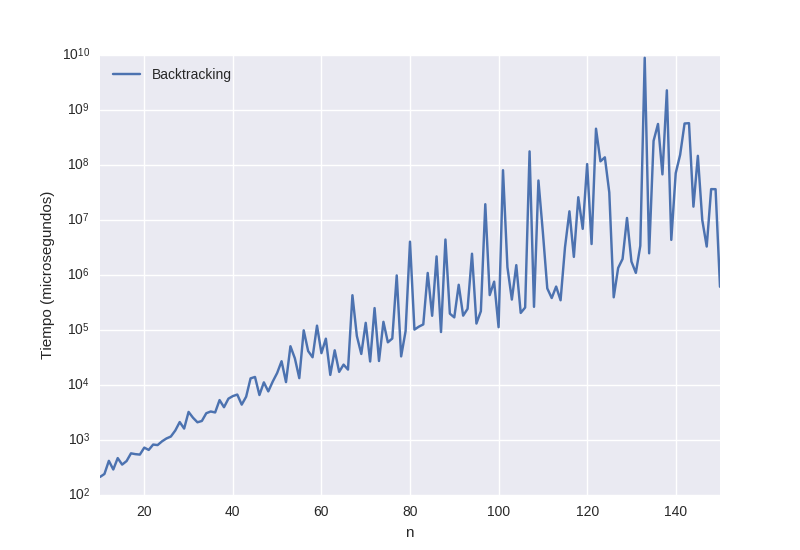
\includegraphics[scale=0.6]{Imagenes/Tiempos150nlogy.png}
		\caption{\small{Tiempos de cómputo del algoritmo exacto según cantidad de nodos.}}
        \label{backtrackingN}
\end{figure}

En la figura \ref{backtrackingN} se puede observar el resultado de las mediciones. Tal como era esperable, los tiempos de cómputo aumentan de forma exponencial según el tamaño de entrada. Sin embargo, presenta variaciones significativas dadas por alguna otra variable. 

Observando algunos de los grafos que llevaron mayor tiempo resolver, notamos que tenían mayor cantidad de aristas ($m$) que sus vecinos en $n$, por lo que analizamos la posibilidad de que la cantidad de aristas afecte de forma más directa a la complejidad del algoritmo que la cantidad de nodos. Esto es posible ya que por como fueron generados los grafos, la relación entre cantidad de nodos y aristas es solo directa en probabilidad, y presenta variaciones aleatorias. En la figura \ref{backtrackingM} se grafican los mismos datos, pero ordenados según cantidad de aristas, y se puede observar que presentan aún más variación que la figura anterior. 

Por lo tanto las variables que afectan a la complejidad del algoritmo, además de $n$ y $m$, deben deberse a alguna otra caractéristica de los grafos más difícil de caracterizar, como puede ser por ejemplo la cantidad total de cliques.

\begin{figure}[h!]
	\centering
		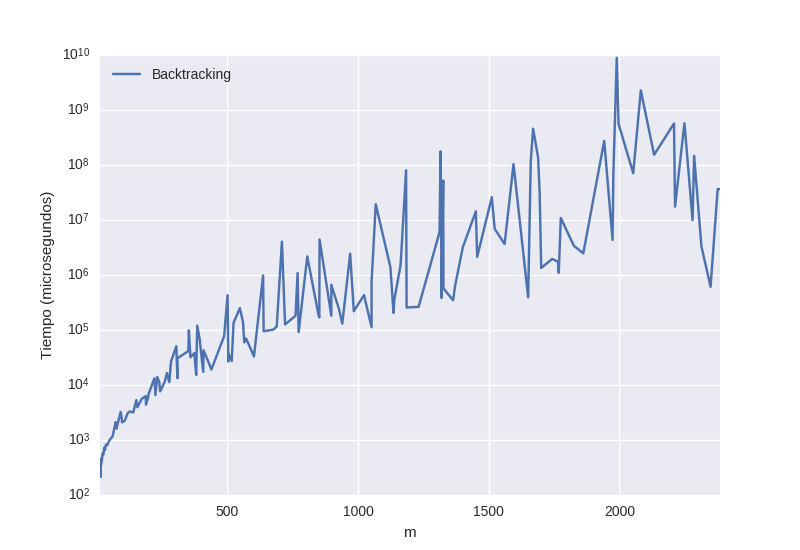
\includegraphics[scale=0.6]{Imagenes/Tiempos150mlogy.png}
		\caption{\small{Tiempos de cómputo del algoritmo exacto según cantidad de aristas.}}
        \label{backtrackingM}
\end{figure}
\newpage

\section{Heurísticas golosas}
\subsection{LFS}

Inspirada en la heurística LFS (\textit{Secualcial Largest First})  esta heurística golosa, o \textit{greedy} funciona de forma iterativa y se basa en la intuición de que un nodo de mayor grado tiene más probabilidades de pertenecer a una clique de frontera maxima. Esto se debe a que como tiene muchas adyacencias, muchas de estas contribuirán al tamaño de la frontera, o en caso de que la mayoría de sus vecinos sean parte de la clique también, será mayor la cantidad de vecinos que aumentan la frontera.

\subsubsection{Algoritmo}

Para implementar esta idea, el primer paso es armar una lista de todos los nodos del grafo, ordenados de mayor a menor según su grado. La solución al problema es una clique representada como un conjunto de nodos.

Comenzando con una clique vacía y por lo tanto de frontera nula como solución parcial, en cada paso iterativo se decide si el próximo nodo es agregado a la solución. Para ser agregado debe cumplir:

\begin{itemize}
\item La solución anterior más el nuevo nodo forman una clique.
\item La clique nueva tiene frontera mayor que la solución anterior.
\end{itemize}

Esta función recorre todos los nodos que pueden ser agregados y devuelve los nodos que forman la clique encontrada y el tamaño de su frontera. El funcionamiento del algoritmo se puede entender mejor viendo el siguiente pseudocódigo:\\


\begin{algorithm}[H]
\begin{algorithmic}
\caption{Algoritmo goloso LFS.}
	\Function{maxFronCliqueLFS}{}
		\State{}
		$nodos \gets$ Vector con los nodos y sus grados \;
		Ordeno $nodos$ de mayor a menor según su grado\;
		$clique \gets$ Vector vacío\;
		$maxFront \gets$ 0\;
		$tamClique \gets$ 0\;
		
		\For{cada i desde 1 hasta n, y mientras $nodos_i$ pueda mejorar la solución }{
			\State{}
			$clique$.Agregar($nodos_i$) \;
			\eIf{$clique$ es clique y tiene mayor frontera que antes}{
				\State{}
				Actualizar($maxFront$) \;
				$tamClique \gets tamClique$ + 1
			}{
				\State{}
				$clique$.Remover($nodos_i$) 
			}
		}
		\Return{$clique$ y $maxFront$}
	\EndFunction
\end{algorithmic}
\end{algorithm}



En este pseudocódigo hay tres operaciones que no son triviales de resolver. Una es verificar que un conjunto de nodos forman efectivamente una clique. Sabiendo que antes de agregar el último nodo ya era una clique, esto se realiza verificando que el último nodo esta conectado con todos los anteriores.

Para entender las otras dos operaciones, que son verificar que $nodos_i$ pueda mejorar la solución y calcular la forntera de $clique$ + $nodos_i$, hace falta demostrar un pequeño lema primero.\\

\textbf{Lema 1:} Sea $C_k$ una clique de $G$ de $k$ nodos, $f(C_k)$ el tamaño de su frontera, y $v'$ un nodo de G tal que $v' \not \in$ $C_k$. Si $C_{k+1} = C_k$ + $v'$ es una clique, $f(C_{k+1}) = f(C_k) + d(v') - 2*k$. \\

\textbf{Demostración:} De forma constructiva podemos ver que al agregar un nodo $v'$ a la clique $C_k$, todas las aristas que unian a $C_k$ con $v'$ dejan de estar en la frontera. Por otro lado, ahora pertenecen a la frontera todas las aristas incidentes a $v'$ que no se conectan con nodos de $C_k$.\\
Como sabemos que $C_{k+1}$ es una clique, tiene que haber exactamente una arista entre cada nodo de $C_k$ y $v'$, por lo que  $f(C_{k+1}) = (f(C_k) - k) + (d(v') - k) = f(C_k) + d(v') - 2*k$.\\


De esta forma es trivial calcular el tamaño de la frontera y, además, se deduce inmediatamente que para que el nodo a añadir agrande la frontera de la clique, debe tener grado mayor a $2*k$. Esto nos ahorra verificar con todo nodo que no cumpla esta condición.

\subsubsection{Complejidad}

En este algoritmo, la complejidad se divide en tres partes: La complejidad del \textit{set up}, la complejidad del ciclo, retornar los resultados.

En la primera parte, inicialmente se genera un vector de pares, donde se coloca cada nodo con su grado. Dado que contruir un par tiene costo $O(1)$, el costo de agregar un par nuevo es el costo de calcular el grado del nodo. Esto se realiza recorriendo la columna de la matriz de adyacencias correspondiente al nodo, contando la cantidad de adyacencias. Al tratarse de una matriz cuadrada de $n x n$, el costo de determinar el grado es $O(n)$. As\'i, como se agrega un par por cada nodo, el costo final de esta operaci\'on es $O(n^2)$.

Una vez obtenido el vector de pares, se lo ordena descendentemente. Debido a que la comparaci\'on entre dos pares se realiza en $O(1)$ (ya que consta en comparar solo la primera componente del par), ordenar los $n$ pares tiene costo $O(n*log(n))$.

En cuanto a la primera parte, solo resta hacer pequeñas asignaciones las cuales no implican un costo adicional. Por lo tanto, el costo total de la primera parte es $O(n^2)$ + $O(n*log(n))$ = $O(n^2)$.

La segunda parte es el cuerpo del algoritmo, el cual está compuesto por un ciclo que, en peor caso, recorre todos los nodos. Determinar si un nodo es candidato para mejorar la solución consiste simplemente en verificar que el grado del nodo es mayor a dos veces tamaño de la clique. Como el grado del nodo ya fue calculado en la primera parte, esta validación tiene costo constante. Así, el ciclo realiza $O(n)$ iteraciones donde el paso de una a otra no implica costo significativo.

En cada iteración primero se agrega un nuevo nodo, lo cual tiene costo $O(1)$, y luego se verifican dos cosas:

\begin{itemize}
\item Que la nueva tira de nodos es clique luego de agregar al último nodo. Como solo es necesario verificar que el último nodo sea adyacente a los anterior (debido a que ya era clique antes de agregar al último nodo) el costo de esta operación es $O(n)$\footnote{ Ver costo de operación $esClique$ en algoritmo de Backtracking.}. 
\item Si se cumple que es clique, se verifica si el tamaño de la frontera es mayor. Esto tiene costo constante utilizando la propiedad mencionada previamente.
\end{itemize}

Una vez realizadas estas verificaciones, el costo restante es constante, independientemente de si se cumple lo anterior o no. De cumplir, solo se guardan los valores nuevos, y si no se cumple, se remueve el nodo agregado, el cual se encuentra siempre en la última posición.

Finalmente, el costo de la segunda parte del algoritmo está dominado por determinar si una tira de nodos es clique en cada iteración, y por lo tanto el costo es $O(n)$ * $O(n)$ = $O(n^2)$.

La tercera y última parte es retornar los resultado. Esto no tiene costo significativo ya que copiar el tamaño máximo de la frontera es constante, y la clique se devuelve por referencia.

Habiendo calculado las tres partes, el costo total en peor caso el la suma de las complejidades de las tres partes. Esto es $O(n^2)$ + $O(n^2)$ + $O(1)$ = $O(n^2)$.

\subsection{Random}

Esta heurística golosa imita la heurística anterior, pero sin considerar ningún orden particular para los nodos. Es claro que, si bien el nodo de mayor grado parece una buena forma de comenzar, éste no siempre formará parte de la solución. Por este motivo, un orden aleatorio resulta una alternativa tentadora a la hora de experimentar.

\subsubsection{Algoritmo}

El algoritmo de esta heurística presenta muy pocas modificaciones con respecto al anterior. La principal es, sin duda, que ya no se ordenan los nodos en base a su grado, sino que se genera una lista con todos los nodos y luego se los mezcla aleatoreamente. Luego, en el cuerpo del algoritmo se busca agregar nodos que mejoren la frontera en el orden provisto por la tira mezclada.

\begin{algorithm}[H]
\begin{algorithmic}
\caption{Algoritmo goloso aleatorio.}
	\Function{maxFronCliqueRandom}{}
		\State{}
		$nodos \gets$ Vector con los nodos\;
		Mezclar(nodos)\;
		$clique \gets$ Vector vacío\;
		$maxFront \gets$ 0\;
		$tamClique \gets$ 0\;
		
		\For{cada i desde 1 hasta n}{
			$clique$.Agregar($nodos_i$)\;
			
			\eIf{$clique$ es clique y tiene mayor frontera que antes}{
				\State{}
				Actualizar($maxFront$) \;
				$tamClique \gets tamClique$ + 1\;
			}{
				\State{}
				$clique$.Remover($nodos_i$) \;
			}
		}
		\Return{$clique$ y $maxFront$} \\
	\EndFunction
\end{algorithmic}
\end{algorithm}

\subsubsection{Complejidad}

Al igual que el algoritmo de LFS, la complejidad se divide en tres partes: La complejidad del \textit{set up}, la complejidad del ciclo, retornar los resultados.

La tercera y última parte se mantiene igual al otro algoritmo, por lo tanto la complejidad es $O(1)$.

En cuanto a las dos primeras partes, ambas sufren algún cambio con respecto a LFS. En la primera parte ya no se calculan todos los grados y luego se ordenan, sino que simplemente se ponen todos los nodos en un vector ($O(n)$) y luego se los mezcla aleatoreamente. Esta última operación tiene orden lineal en la cantidad de elementos del vector, por lo tanto, la complejidad final de la primera parte es $O(n)$ + $O(n)$ = $O(n)$.

En cuanto a la segunda parte, los cambios que se realizan son muy sutiles. El primero es que, al no tener los grados de los nodos calculados, ya no se puede evitar considerar unos de los nodos por tener grado muy bajo. Esto hace que se recorran todos los nodos hasta el final de la lista. De todas formas, en peor caso, esto no altera la complejidad. Se siguen realizando $O(n)$ iteraciones. El segundo cambio que se realiza es a la hora de calcular la nueva frontera de la clique. Como antes se tenían calculados los grados de los nodos, este cálculo resultaba tener costo constante. En este algoritmo, en cambio, hay que calcularlo con costo $O(n)$. De todas formas, como previamente se debe calcular si la tira de nodos es efectivamente una clique en $O(n)$, el costo final de esta parte no se ve afectado. Al igual que en LFS, lo restante es de orden constante. 

 Así, la complejidad del cuerpo del algoritmos $O(n)$ * $O(n)$ = $O(n^2)$, y sumando a esto el costo de la primera parte o \textit{set up}, la complejidad final del algoritmos es $O(n^2)$ + $O(n)$ = $O(n^2)$, al igual que el algoritmo de LFS.

\subsection{Experimentación}
\newpage

\section{Heurísticas de búsqueda local}
\subsection{Algoritmo}
En la búsqueda local intentaremos mejorar una solución inicial moviéndonos en una vecindad chica de esta solución, es decir, analizaremos soluciones que distan a lo sumo un nodo de la solución original buscando encontrar una clique de máxima frontera local.

Para ello, se le aplicarán 3 operaciones a una solución, las cuales consisten en:

\begin{enumerate}
\item Agregar un nodo vecino a la clique a la solución 
\item Eliminar un nodo de la clique solución
\item Intercambiar un nodo de la solución por un nodo vecino a la clique
\end{enumerate}

Para cada una de estas operaciones, siempre se elegirá modificar la solución de forma que se maximice la CMF obtenida de entre las posibles modificaciones a realizar.

A continuación se detallarán las operaciones mencionadas anteriormente para una mejor comprensión.

Mejorar la solución agregando un nodo consiste en ver para cada nodo vecino de la clique si al agregarlo a la solución, ésta sigue siendo una clique. En caso de ser una clique se calculará su frontera y se verá si mejora la frontera con respecto a la solución inicial y con los nodos vecinos que se verificó anteriormente. Luego se quitará el nodo agregado para seguir probando con el resto de los vecinos. Finalmente se agregará el nodo vecino que más mejore la frontera de la clique, de no existir ninguno que la mejore no se agregará nada.

\begin{algorithm}[H]
\begin{algorithmic}
\caption{Mejora la solución agregando un nodo vecino}
	\Function{mejorarAgregando}{Matriz de adyacencias, n, cliqueMF, maxFront}
		\State{}\\
		vecinos $\leftarrow$ dameVecinosClique(Matriz de adyacencias, n, cliqueMF)\\
		\For{i entre 0 y tamaño de vecinos}{
			\State{}\\
			Agregar $vecinos_i$ a la cliqueMF
			\If{Sigue siendo una clique y tiene mayor frontera que maxFront}{
				\State{}\\
				Actualizar(maxFront)\\
				mejorNodo $\leftarrow$ $vecinos_i$
			}
			Eliminar $vecinos_i$ de la cliqueMF
		}
		\If{Si agregar algun nodo mejora la frontera}{
			\State{}\\
			Agregar $mejorNodo$ a la clique
		}
	\EndFunction
\end{algorithmic}
\end{algorithm}


Mejorar la solución eliminando un nodo toma un nodo de la clique y lo elimina de la solución, calcula la frontera de esa nueva clique y ve si mejora con respecto a la mejor solución obtenida hasta el momento. Luego vuelve a agregar el nodo eliminado para verificar el resto. Finalmente se elimina el nodo que más mejora la frontera al eliminarlo, si no existe ninguno que mejore no se eliminará ningún nodo.

\begin{algorithm}[H]
\begin{algorithmic}
\caption{Mejora la solución eliminando un nodo de la clique}
	\Function{mejorarEliminando}{Matriz de adyacencias, n, cliqueMF, maxFront}
		\State{}\\
		\For{i entre 0 y tamaño de cliqueMF}{
			\State{}\\
			nodoEliminado $\leftarrow$ cliqueMF[0]
			Eliminar primer elemento de cliqueMF
			\If{tiene mayor frontera que maxFront}{
				\State{}\\
				Actualizar(maxFront)\\
				mejorNodo $\leftarrow$ $nodoEliminado$
			}
			Agregar atras $nodoEliminado$ a la cliqueMF
		}
		\If{Si eliminar algun nodo mejora la frontera}{
			\State{}\\
			Eliminar $nodoEliminado$ de la clique
		}
	\EndFunction
\end{algorithmic}
\end{algorithm}

Mejorar la solución intercambiando un nodo por otro puede considerarse una combinación de las operaciones anteriores dado que en primer lugar se elimina un nodo de la clique y luego se busca cuál es el nodo vecino a la clique que más mejora la frontera al agregarlo. Luego se vuelve a agregar el nodo eliminado y se repite el mismo procedimiento eliminando a cada nodo de la clique. Finalmente se aplicará la operacion de eliminar un nodo de la clique y agregar un nodo vecino que más mejore la frontera, si no hay operación que mejore no se hará nada.

\begin{algorithm}[H]
\begin{algorithmic}
\caption{Mejora la solución intercambiando un nodo de la clique por un vecino}
	\Function{mejorarIntercambiando}{Matriz de adyacencias, n, cliqueMF, maxFront}
		\State{}\\
		\For{i entre 0 y tamaño de cliqueMF}{
			\State{}\\
			nodoEliminado $\leftarrow$ cliqueMF[0]\\
			Eliminar primer elemento de cliqueMF\\
			vecinos $\leftarrow$ dameVecinosClique(Matriz de adyacencias, n, cliqueMF)\\
			\For{j entre 0 y tamaño de vecinos}{
				agregar $vecinos_i$ a la clique\\
				\If{es clique y tiene mayor frontera que maxFront}{
					\State{}\\
					Actualizar(maxFront)\\
					mejorNodo $\leftarrow$ $vecinos_i$\\
				}
				Eliminar $vecinos_i$ de la clique\\
			}
			Agregar atras $nodoEliminado$ a la cliqueMF\\
		}
		\If{Si intercambiar algun nodo mejora la frontera}{
			\State{}\\
			Eliminar $nodoEliminado$ de la clique\\
			Agregar $mejorNodo$ a la clique\\
		}
	\EndFunction
\end{algorithmic}
\end{algorithm}

Ahora nos queda describir cómo usa la búsqueda local estas operaciones, el comportamiento es bastante sencillo, primero se obtiene una solución inicial mediante el algoritmo greedy LFS descripto en la sección de heurísticas golosas. Luego, se ingresará a un ciclo que continuará mientras se siga mejorando la solución. En este ciclo se aplicarán las 3 operaciones de agregar, eliminar e intercambiar nodos a la solución obtenida hasta el momento pero solo se mantendrá la operación que mas mejoró la solución, si ninguna operación pudo mejorar la solución se considera que se llegó a una solución óptima local por lo que se saldrá del ciclo finalizando el algoritmo.

Se puede ver de forma más clara el funcionamiento de búsqueda local en el siguiente pseudocódigo:

\begin{algorithm}[H]
\begin{algorithmic}
\caption{Búsqueda local}
	\Function{BusqLocal}{Matriz de adyacencias, n, cliqueMF}
		\State{}\\
		res $\leftarrow$ maxFronCliqueLFS(Matriz de adyacencias, n, cliqueMF)\\
		CMFAgregar $\leftarrow$ Vacio\\
		CMFEliminar $\leftarrow$ Vacio\\
		CMFIntercambiar $\leftarrow$ Vacio\\
		\While{Sigue mejorando la solución}{
			\State{}\\
			CMFAgregar $\leftarrow$ cliqueMF
			CMFEliminar $\leftarrow$ cliqueMF
			CMFIntercambiar $\leftarrow$ cliqueMF
			resAgregar $\leftarrow$ mejorarAgregando(Matriz de adyacencias, n, CMFAgregar, res)\\
			resEliminar $\leftarrow$ mejorarEliminando(Matriz de adyacencias, n, CMFEliminar, res)\\
			resIntercambiar $\leftarrow$ mejorarIntercambiando(Matriz de adyacencias, n, CMFIntercambiar, res)\\
			Actualizar $res$ y $cliqueMF$ con la operación que más mejore la solución\\
			Si ninguna operación mejora, se sale del ciclo
		}
	\EndFunction
\end{algorithmic}
\end{algorithm}

\subsection{Complejidad}

Para calcular la complejidad del algoritmo podemos dividirlo en 3 partes: la complejidad del \textit{set up}, la complejidad del ciclo y retornar el resultado.

En el \textit{set up} se crean 3 vectores vacíos con costo $O(1)$ y se ejecuta el algoritmo $maxFronCliqueLFS$ que como ya se demostro tiene complejidad $O(n^2)$. Por lo tanto está parte tiene complejidad $O(n^2)$.

En la segunda parte, que es el ciclo del algoritmo podemos analizar primero la complejidad de las operaciones dentro del mismo.

En primer lugar se copia la CMF a 3 vectores auxiliares con costo $O(n)$ para cada uno.

Se ejecuta $mejorarAgregando$ que utiliza la funcion $dameVecinosClique$ con costo $O(n^3)$. Luego se inicia un ciclo que realizará n iteraciones en el peor caso donde en cada iteración se ve si agregar un nodo a la clique hace que ésta siga siendo una clique con costo $O(n)$ y se calcula su frontera con costo $O(n^2)$. Por lo tanto la complejidad del algoritmo es $O(n^3)$ + $O(n)$ * ($O(n)$ + $O(n^2)$) = $O(n^3)$

Se ejecuta mejorarEliminando que comienza con un ciclo que realizará n iteraciones en el peor caso, dentro del ciclo se eliminará el primer elemnto de un vector con costo $O(n)$ y se calculará su frontera con costo $O(n^2)$. Una vez fuera del ciclo se buscará el nodo a eliminar en el vector con costo $O(n)$ y luego se lo eliminará también con costo $O(n)$. Entonces, la complejidad del algoritmo queda como $O(n)$ * ($O(n^2)$ + $O(n)$) + $O(n)$ * $O(n)$ = $O(n^3)$

También se ejecuta mejorarIntercambiando que tiene 2 ciclos anidados con una particularidad: el peor ciclo de uno de los ciclos garantiza que el otro ciclo está en su mejor caso. 

En el caso de que el ciclo externo realice $n$ iteraciones significa que la clique es de tamaño $n$, dentro de este ciclo se eliminará el primer elemento de la clique con costo $O(n)$ y se calcularán sus vecinos con costo $O(n^3)$. Ahora, como la clique tiene tamaño $n$ no puede tener vecinos que no pertenezcan a la clique por lo que este vector estará vació. Debido a esto el ciclo interno no realizará ninguna iteración y luego se agregará el nodo eliminado nuevamente con costo $O(1)$. La complejidad de esto será entonces $O(n)$ * ($O(n)$ + $O(n^3)$) = $O(n^4)$

En el caso contrario de que la clique sea lo más chica posible, es decir, de tamaño 2 ya que sino al eliminar un nodo queda una clique vacía, el ciclo externo realizará 2 iteraciónes. Eliminará el primer nodo con costo $O(1)$ y calculará sus vecinos con costo $O(n^3)$, la cantidad de vecinos puede ser a lo sumo $n-1$ por lo que el ciclo interno puede llegar a realizar $n-1$ iteraciones. Dentro del ciclo interno se agrega un nodo con costo $O(1)$, se verifica que siga siendo clique al agregarlo con costo $O(n)$ y se calcula su frontera con costo $O(n^2)$. Luego se elimina el último elemento agregado con costo $O(1)$. La complejidad de esto será entonces $O(2)$ * ($O(n^3)$ + $O(n)$ * $O(n)$ + $O(n^2)$) = $O(n^3)$

Finalmente luego de estos ciclos anidados en el caso de que exista algun intercambio que mejore la solución se busca el nodo que hay que eliminar y se lo elimina con costo $O(n^2)$ y luego se agrega otro nodo con costo $O(1)$.

La complejidad de $mejorarIntercambiando$ será entonces $O(n^4)$ + $O(n^3)$ $O(n^2)$ = $O(n^4)$

Luego de ejecutadas las 3 operaciones, se elegirá cual es la que conviene con costo $O(1)$ y se actualizará la clique con costo $O(n)$. Por lo tanto la complejidad interna del ciclo es $O(n)$ + $O(n^3)$ + $O(n^3)$ + $O(n^4)$ + $O(n)$ = $O(n^4)$

Ahora nos queda ver cuantas iteraciones realiza el ciclo. Dado que depende de que la solución continúe mejorando para seguir ejecutando el ciclo analizaremos hasta cuando puede mejorar la solución. Un grafo siempre tiene una frontera mayor o igual a 0 y menor o igual a la cantidad de aristas $m$. Como $m$ $\leq$ $n^2$ una cota para la cantidad de mejoras que se pueden hacer a una solución es $n^2$. Sin embargo, como las operaciones de mejora trabajan sobre nodos y no sobre aristas veremos que esta cota nunca se alcanza.

Si se partiera de una clique de tamaño 1 y la solución óptima fuera el grafo completo, se agregarán $n-1$ nodos por lo que el ciclo realizará $n-1$ iteraciones.

Si se parte de una clique que es el grafo completo y la clique óptima tuviera tamaño 1, se eliminarán n-1 nodos por lo que el ciclo también realizará $n-1$ iteraciones.

De forma más global se puede ver que si un nodo fue agregado a la solución no puede ser eliminado en las proximas iteraciones dado que no mejoraría la solución. Lo mismo sucede si se eliminó un nodo, al vovler a agregarlo se estaría empeorando la misma. Como el intercambio es una combinación de agregar y eliminar también se ve que no se podrían realizar varias operaciones sobre un nodo.

De este razonamiento podemos concluir que a cada nodo del grafo se le puede aplicar a lo sumo 1 operación de las 3 mencionadas de forma que mejore la solución. Entonces, a lo sumo se realizan $n$ mejoras a la ssolución. Por lo tanto el ciclo realizará a lo sumo $n$ iteraciones.

Entonces la complejidad del ciclo sera $O(n)$ * $O(n^4)$ = $O(n^5)$

La tercera y última parte es retornar los resultados. Esto no tiene costo significativo ya que copiar el tamaño máximo de la frontera es constante, y la clique se devuelve por referencia.

Podemos concluir entonces que la complejidad de la búsqueda local será entonces $O(n^2)$ + $O(n^5)$ + $O(1)$ = $O(n^5)$
\newpage

\section{Metaheurísticas}
\subsection{Algoritmo}
Dado que ninguna heurística garantiza soluciones de calidad para cualquier tipo de grafo, en este algoritmo nos concentraremos en utilizar las heurísticas de forma inteligente intentando que la solución brindada sea siempre de buena calidad sin importar el grafo que se establece en la entrada.

Para ello nos basaremos en el algoritmo de GRASP (Greedy randomized adaptive search procedure) el cual genera soluciones greedys partiendo desde distintos nodos del grafo buscando cubrir la mayor cantidad de soluciones posibles devolviendo finalmente la mejor solución.

Una parte fundamental de GRASP es el algoritmo que genera las soluciones greedy aleatorias, dado que debe de poder generar soluciones lo suficientemente diferentes para que se garantice explorar un amplio espectro del espacio de soluciones.

En nuestro algoritmo, nuestra solución aleatoria se construye eligiendo un nodo al azar de una lista de nodos que no fueron utilizados en las últimas $n$ soluciones y luego agregando sus vecinos que más mejoren la solución. Se puede ver cómo funciona el algoritmo en el siguiente pseudocódigo:

\begin{algorithm}[H]
\begin{algorithmic}
\caption{Algoritmo greedy aleatorio}
	\Function{CMFRandomGreedy}{Matriz de Adyacencias, n, cliqueMF}
		\State{}\\
		\If{NoUsados es Vacio}{
			\State{}\\
			\For{Desde i entre 1 y n}{
				\State{}\\
				noUsados $\leftarrow$ AgregarAtras(noUsados, i)\\
			}
			noUsados $\leftarrow$ Mezclar(noUsados)
		}
		nodo $\leftarrow$ Ultimo(noUsados)\\
		noUsados $\leftarrow$ EliminarUltimo(noUsados)\\
		clique $\leftarrow$ Vacio\\
		clique $\leftarrow$ AgregarAtras(clique, nodo)\\
		maxFront $\leftarrow$ TamFrontera(clique)\\
		tamClique $leftarrow$ 1\\
		vecinos $\leftarrow$ dameVecinosCliqueyGrado(clique)\\
		vecinos $\leftarrow$ OrdenarporGrado(Vecinos)\\
		\For{i desde 1 hasta Tamaño(vecinos) y mientras $vecinos_i$ pueda mejorar la solución}{
			\State{}\\
			clique $\leftarrow$ AgregarAtras($vecinos_i$, clique) \\
			\\
			\If{$clique$ es clique y tiene mayor frontera que antes}{
				\State{}\\
				Actualizo $maxFront$ \\
				tamClique $\leftarrow$ tamClique + 1\\
			}
			\Else{
				\State{}\\
				clique $\leftarrow$ EliminarUltimo(clique)\\ 
			}			
		}
		cliqueMF $\leftarrow$ clique\\
		\Return{$maxFront$} \\
	\EndFunction
\end{algorithmic}
\end{algorithm} 

Se analizará en la experimentación las mejoras en rendimiento y calidad de soluciones que se obtendrán al modificar este algoritmo.

Otra parte importante de GRASP es cuándo termina el algoritmo, es decir, cuándo consideramos que ya buscó una cantidad suficientemente buena de soluciones diferentes por lo que ya deberíamos obtener una solución de buena calidad con alta probabilidad. Ńuestro algoritmo terminará luego de buscar una cantidad de soluciones sin que se mejore la mejor solución obtenida hasta el momento. Esta cantidad de iteraciones sin mejorar la solución se determinará en la entrada y se verá luego las variaciones en el rendimiento y en las soluciones que se obtienen al modificar este valor.

Finalmente, el algoritmo de GRASP que realizamos se puede resumir de la siguiente forma:

\begin{algorithm}[H]
\begin{algorithmic}
\caption{Algoritmo GRASP}
	\Function{CMFGRASP}{Matriz de Adyacencias, n, cliqueMF, limite}
		\State{}\\
		maxFront $\leftarrow$ maxFronCliqueLFS(Matriz de adyacencias, n, cliqueMF)\\
		maxFrontAux $\leftarrow$ 0\\
		CMFAux $\leftarrow$ Vacio\\
		iterSinMejorar $\leftarrow$ 0\\
		\While{iterSinMejorar < limite}{
			\State{}\\
			maxFrontAux $\leftarrow$ CMFRandomGreedy(Matriz de Adyacencias, n, CMFAux)\\
			maxFrontAux $\leftarrow$ MejorarBusqLocalVecChica(Matriz de Adyacencias, n, CMFAux, maxFrontAux)\\
			\If{maxFrontAux > maxFront}{
				\State{}\\
				maxFront $\leftarrow$ maxFrontAux\\
				Actualizo cliqueMF\\
			}
			\Else{
				iterSinMejorar $\leftarrow$ iterSinMejorar + 1\\
			}
			Vaciar(CMFAux)\\
		}
		\Return{$maxFront$} \\
	\EndFunction
\end{algorithmic}
\end{algorithm} 

\subsection{Complejidad}

Vamos a analizar la complejidad del algoritmo dividiendo el algoritmo en partes. En primer lugar comenzaremos con la inicialización de variables donde se crean vectores vacíos y enteros con costo $O(1)$ salvo por el llamado a $maxFronCliqueLFS$ el cual tiene un costo de $O(n^2)$. La complejidad de esta parte será entonces $O(n^2)$

Luego estaremos en el ciclo, comenzaremos por ver el costo de las operaciones dentro del mismo.

 Se llama a la función $CMFRandomGreedy$ la cual inicia llenando un vector vacío con $n$ nodos con costo $O(n)$ y luego mezcla los elementos del mismo también con costo $O(n)$. Se realizan asignaciones y se elimina el último elemento de un vector con costo $O(1)$. Se calcula la frontera de la clique de tamaño 1 generada hasta el momento con costo $O(n)$, se buscan los vecinos de la clique y su grado con costo $O(n^2)$ dado que la clique tiene un solo nodo. Se ordenan los vecinos de forma decreciente según su grado en $O(n log n)$. Luego se ingresa a un ciclo que realizará a lo sumo $n$ iteraciones donde la única operación que no es elemental es ver si se forma una clique al agregar un nodo que tiene costo $O(n)$. Al salir del ciclo se copia la mejor solución en $O(n)$. Por lo tanto la complejidad de $CMFRandomGreedy$ sera $O(n)$ + $O(n)$ + $O(1)$ + $O(n^2)$ + $O(n log n)$ + $O(n)$ * $O(n)$ + $O(n)$ = $O(n^2)$.

 Se llamará a la búsqueda local para la que ya se mostró que tiene complejidad $O(n^5)$

 Luego se copiará la solución obtenida en esta iteración si mejora la mejor solución con costo $O(n)$.

 Nos queda ver cuantas iteraciones hará a lo sumo este ciclo, por un lado depende de un parámetro $l$ que se establece en la entrada que indica cuantas iteraciones realizará el ciclo sin que se mejore la solución, por el otro lado debemos saber cuantas iteraciones se pueden hacer mejorando la solucion, por la forma en que funciona $CMFRandomGreedy$ puede generar $n$ soluciones distintas por lo que luego de $n$ iteraciones donde se mejore siempre la solución es imposible que se siga mejorando. Por lo tanto el ciclo hace a lo sumo $n + l$ iteraciones.

 Entonces el costo total del ciclo será de $O(n + l)$ * ($O(n^2)$ + $O(n^5)$ + $O(n)$) = $O((n+l) * n^5)$

 Finalmente se devuelve la solución con costo $O(1)$

 Concluimos que la complejidad total del algoritmo será de $O(n^2)$ + $O((n+l) * n^5)$ + $O(1)$ = $O((n+l) * n^5)$



\newpage

\section{Experimentación}
\input{6Experimentacion.tex}
\newpage

\section{Conclusión}
\input{7Conclusion.tex}
\end{document}
